\subsection{Initial State for Plasma Formation and Low-$x$ Phenomena}


\begin{figure}[h!]
\centerline{
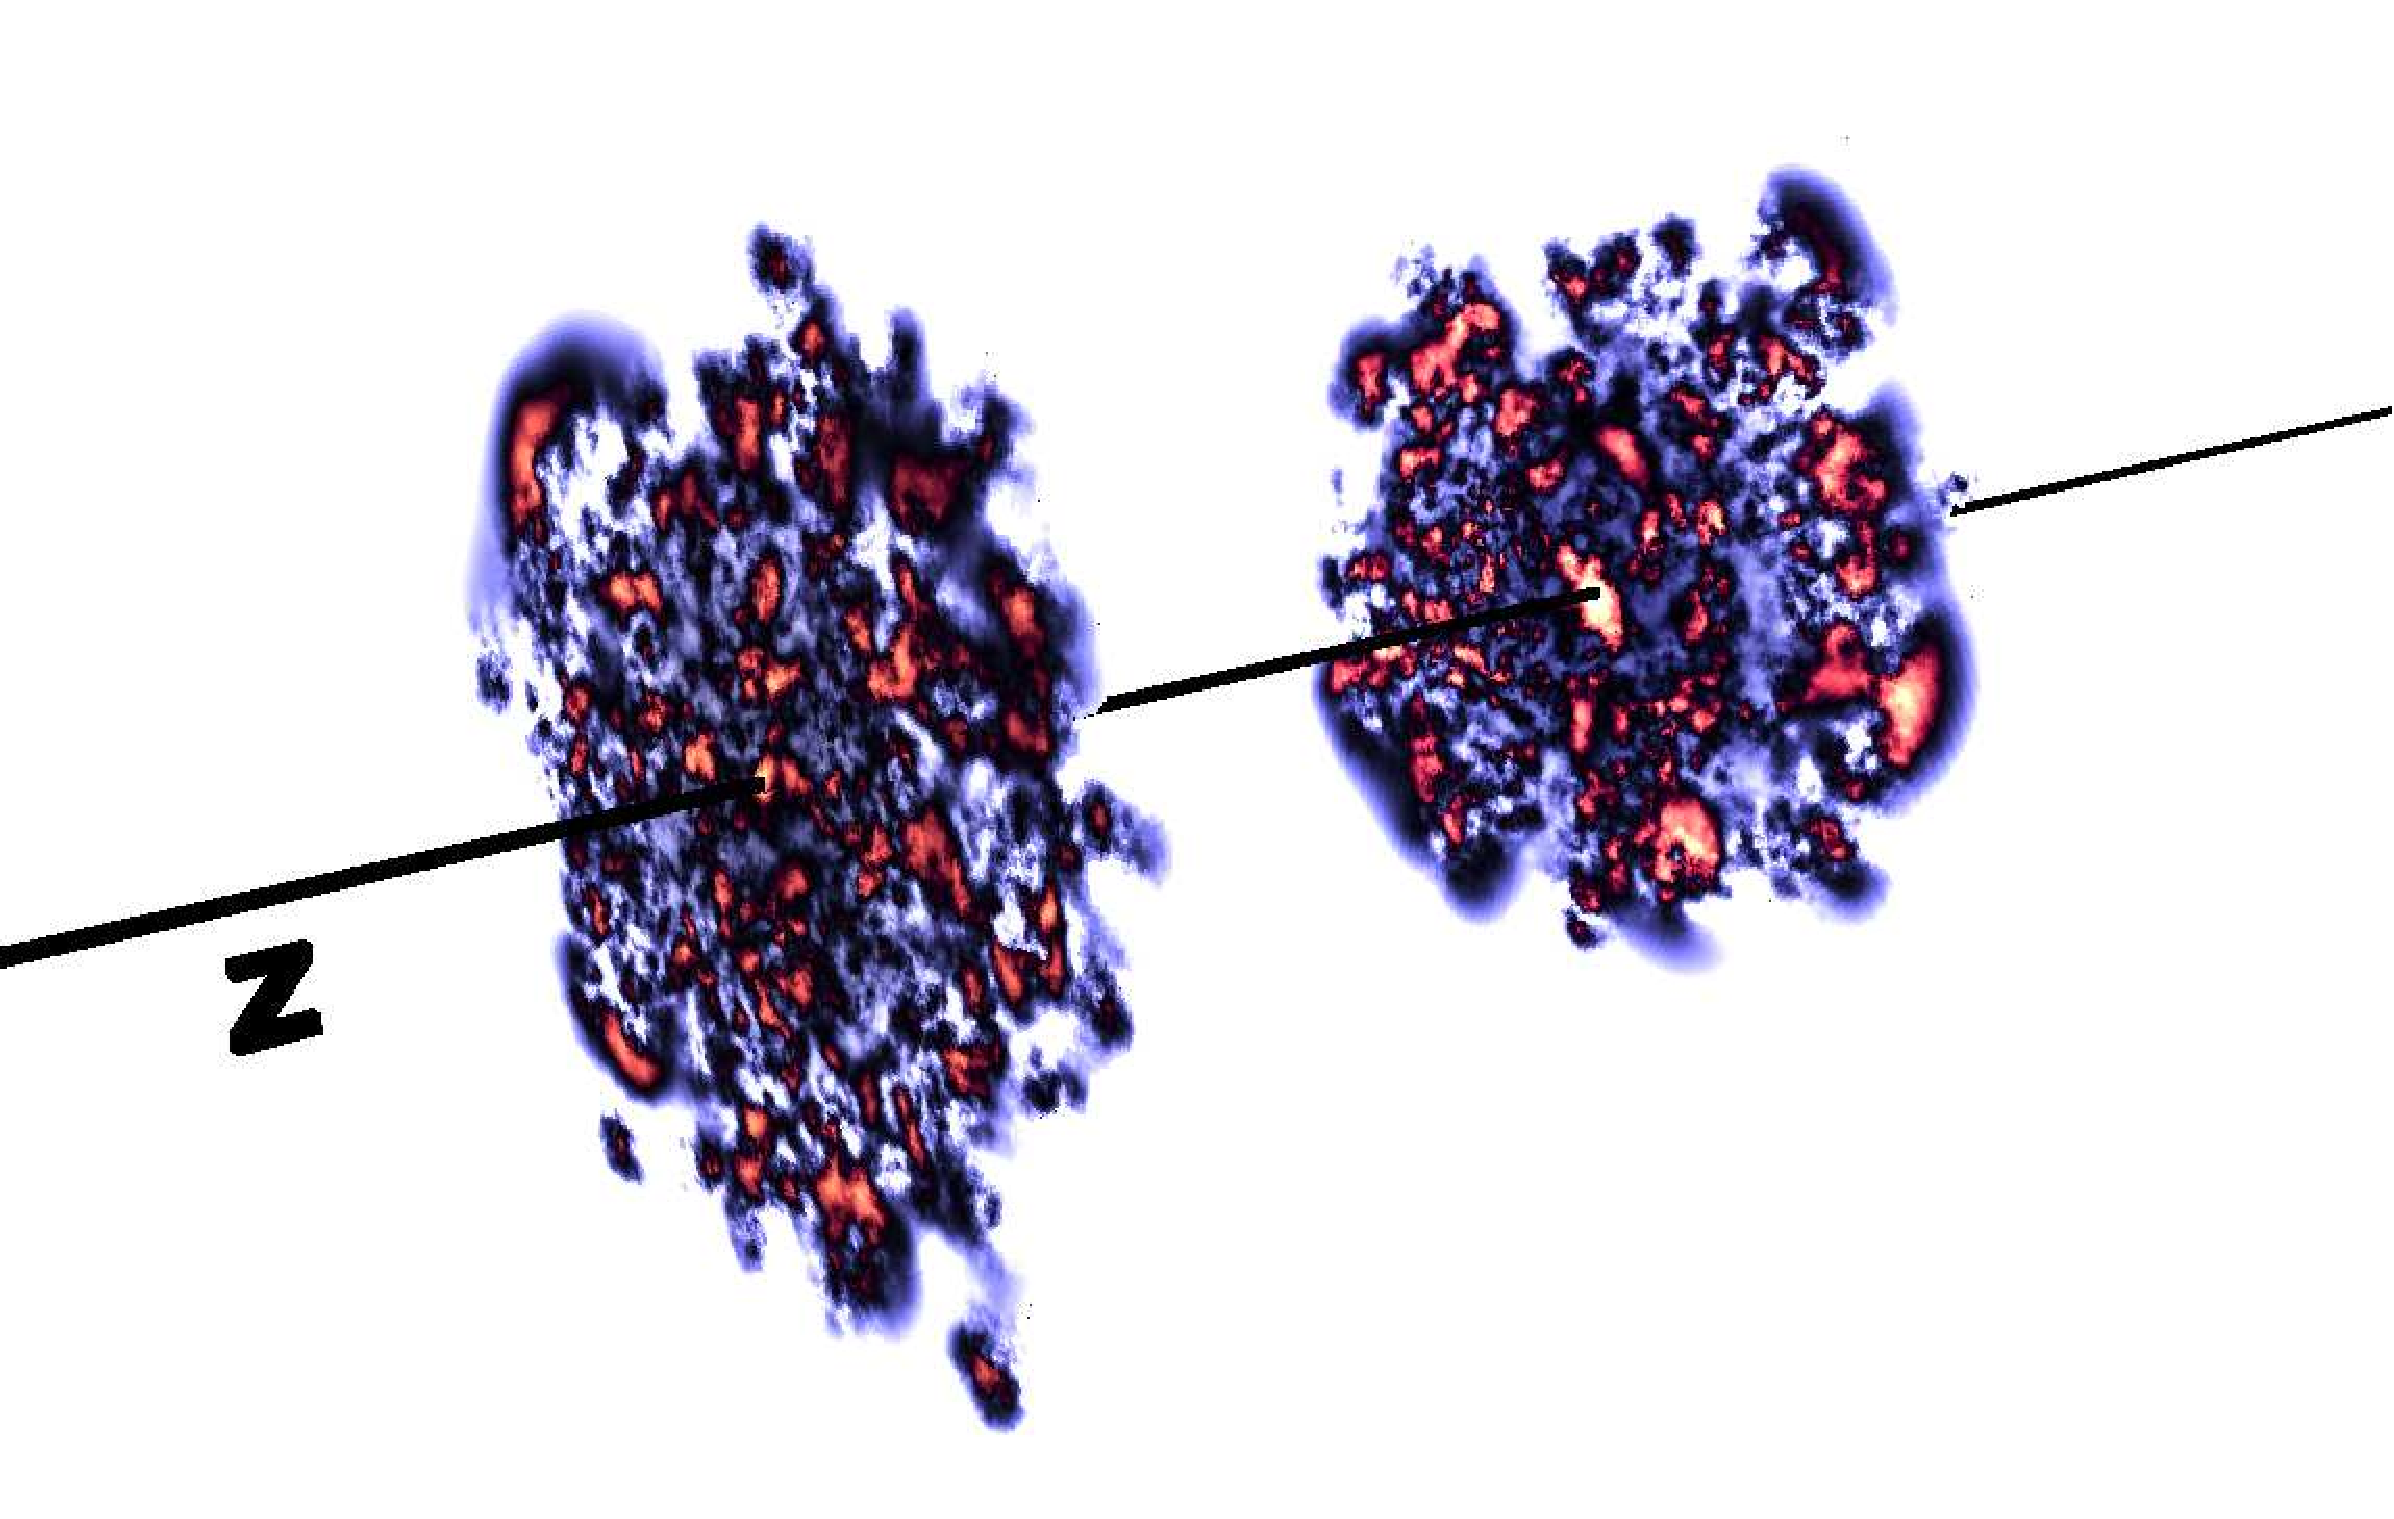
\includegraphics[width=0.75\textwidth]{fig/wVdagVLHC}}
\caption[Color fields of the two nuclei before the collision]{Color fields of the two nuclei before the collision,
from~\cite{Schenke:2012fw}}
\label{fig:colorfield}
\end{figure}

\label{Sec:Saturation}


At the high collision energies of RHIC and the LHC, the  phase space available for radiating small-$x$ 
gluons and quark-antiquark pairs is very large. Since each emitted parton is itself a source of 
additional gluons, an exponentially growing cascade of radiation is created which would 
eventually violate unitarity. However, when the density of partons in the transverse plane
becomes large enough, softer partons begin to recombine into harder ones and the gluon 
density saturates. This limits the growth of the cascade  and preserves the 
unitarity of the $S$-matrix. 
The transverse momentum scale below which these nonlinear interactions dominate is known as 
the \emph{saturation scale} \qs . The saturation scale grows with collision energy, but also with the
size of the nucleus as $\qssqr \sim A^{1/3}$. For high enough energies \qs\ is large and
the corresponding QCD coupling weak $\as(\qs) \ll 1$. This makes it possible to calculate 
even bulk particle production using weak coupling methods, although the calculation is still  nonperturbative due to the large field strengths. Because the gluonic states have large 
occupation numbers, the fields behave 
classically. The classical field theory describing the saturation domain is
known as the ``Color Glass Condensate'' (CGC)~\cite{Gelis:2010nm}. 

The ideal probe of the CGC state are dilute-dense collisions, where a simple small
projectile collides with a large nucleus. At RHIC and the LHC proton-nucleus 
collisions provide such a tool for understanding saturation phenomena. 
Significant progress has been made in describing
the systematics of particle production as a function of transverse momentum and rapidity
in proton-proton and proton-nucleus collisions with CGC 
calculations~\cite{Albacete:2012xq,Tribedy:2011aa,Lappi:2013zma,Fujii:2013gxa,Kang:2013hta}, which are consistent with  the 
collinearly factorized perturbative QCD description~\cite{Helenius:2012wd} at high transverse momenta. 
The case of saturation effects in the multiparticle correlations as a function of azimuthal
angle and rapidity discussed in Section~\ref{Sec:Flow} remains more open. While there are contributions to these correlations 
that originate already in the nuclear wavefunctions~\cite{Dusling:2013oia}, experimental 
evidence points to strong collective behavior also in the final state of 
proton-nucleus and even proton-proton collisions. 
The versatility
of RHIC to systematically change the size of the projectile nucleus
and complement p+A with d+A, $^3$He+A etc. collisions over a wide
range of collision energies is unparalleled and a key to exploring
where these collective effects turn on.  

Yet another approach to probe the nuclear wave-function is provided by virtual photons
produced in ultra-peripheral \pA\ and \AplusA\ collisions. 
Such measurements are sensitive to the gluon structure of the nucleus at low $x$
as well as to cold nuclear matter absorption effects on produced hadrons such as the \Jpsi\ .
At RHIC studies have been of made of $\rho(1700$ production\cite{Abelev:2009aa}
and of coherent production of \JPsi\ 's and high-mass $e^+e^-$ pairs\cite{Afanasiev:2009hy}.
Much higher virtual photon fluxes are provided by the higher collision energies of the LHC, where detailed 
studies have explored the role of gluon shadowing 
in photoproduction of \JPsi\ 's in both \pPb\ \cite{TheALICE:2014dwa} and \PbPb\ collisions\cite{Abelev:2012ba,Abbas:2013oua,CMS:2014ies},
demonstrating sensitivities to Bjorken-$x$ values in both the proton and the Pb nucleus down to $x \sim 10^{-5}$.

 
 

Significant further insight into the structure of high energy nuclei
can be obtained from a polarized p+A program uniquely provided by RHIC\cite{Aschenauer:2015eha}.  
For example, it has been 
suggested~\cite{Kang:2011ni,Kovchegov:2013cva}
that comparing transverse single spin asymmetries measured in polarized p+p
and polarized p+A collisions for different nuclei and at different beam
energies could be very sensitive to the saturation scale $\qs$.
Further, as noted, proton-nucleus collisions have also provided surprises in their own right --- we now understand the resolution of these to be sensitive to the detailed spatial structure of partons in both protons and heavier nuclei. 
The importance of a polarized p+A program is therefore two-fold: (i) It will provide unique and essential information on the parton structure of proton and nuclear wave functions. (ii) The  implementation of this information in models of heavy-ion collisions will provide more sensitive  tests of and precise extraction of the parameters of the Little Bang Standard Model.
Precise and controlled access
to the high energy nucleus is needed to disentangle the effects of
strong collectivity in the initial wave functions and the final
state. An ideal complement to a polarized p+A program will be an Electron-Ion 
Collider that can measure the transverse and longitudinal 
structure of the small-$x$ gluons in nuclei.

Studying both electron-nucleus and proton-nucleus collisions will allow the direct comparison 
of a color neutral to a colored probe of the nuclear medium~\cite{Accardi:2012qut}.
In electron-nucleus collisions,
the parton kinematics are well measured. Furthermore, viewed in the appropriate
Lorentz frame,  the target is probed with a quark-antiquark dipole, which is 
theoretically well-controlled and tunable.
In proton-nucleus collisions, on the other hand, coherent multiple scattering effects
are more complicated.
The combination of data from electron-nucleus and proton-nucleus collisions
is needed to separate
the structure of the medium from the dynamics of the probe. 
The effect of the cold QCD medium on a colored probe must be consistent with theoretical
descriptions developed for partonic interactions in a hot and dense QCD medium.
Thus electron-nucleus and proton-nucleus collisions also 
provide an important control experiment for our theoretical understanding of jet quenching.


The theoretical description of the initial stage of quark-gluon plasma formation has become 
increasingly detailed. State of the art calculations~\cite{Gale:2012rq,Paatelainen:2013eea} 
now combine a 
fluctuating nuclear geometry with a microscopic QCD description of the dynamics of matter
formation that is consistent with our understanding of proton-nucleus collisions 
and deep inelastic scattering. This 
extends the description of the initial state geometry well beyond that provided
by Glauber modeling at the nucleonic level. As discussed in Section~\ref{Sec:Flow}, these initial state 
calculations, combined with detailed measurements of correlations and fluctuations in the
observed flow patterns, have 
helped 
to significantly improve the precision of the first quantitative experimental 
determinations of e.g. the viscosity/entropy ratio $\eta/s$. 

%Due, however, to uncertainties
%in the many stages of modeling 
%the collision process the precision of the extracted QCD matter properties still
%has room for improvement. 
%Further systematic theoretical work,
%together with precise measurements from an Electron-Ion collider, are needed to remove the remaining uncertainties and extend this program to further understand the properties of hot QCD matter. 
